\section{図の挿入}
\LaTeX で図を挿入するというと,以前は EPS形式にする必要があった.
しかし,現在は PDF形式を扱うのが主流である.
したがって,自分で作図した場合は PDF形式にて出力保存するのが適当であろう.
なお,JPEGでもPNGでも挿入は可能なため,デジタルカメラの画像などは PDFに変換する必要は無い.

\subsection{挿入方法}
PDFが主流とはいえ,EPS形式の貼り付けが基本であるため,その方法をまず記述する.

図を入れたいところで以下の様に指定する.
\begin{breakbox}
{\small
\begin{verbatim}
\begin{figure}[htbp]
\centering
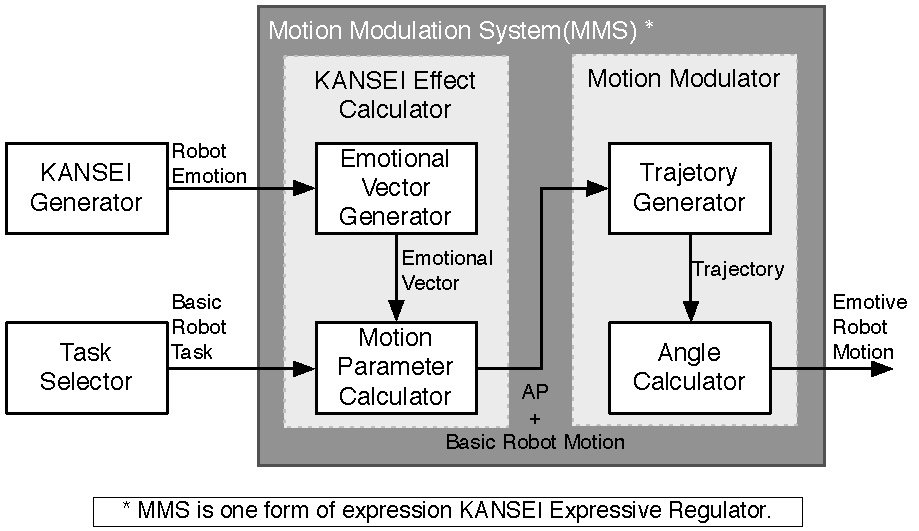
\includegraphics[height=7cm]{MMS.pdf}
\caption{MMSの内部構成}
\label{fig:mms}
\end{figure}
\end{verbatim}
}
\end{breakbox}

\verb+\caption{}+内には,図のタイトルや説明文章を書く(図番号の後ろの部分).
宮治研の場合は,必ず記載すること.
なお,このフォーマットを守る限り気にする必要は無いが,図のタイトルは図の下につけなければならない.

また,\verb+\label{}+は図番号を参照する際のラベルである(使い方は後述).
当然,図毎にラベルの名称を変えなければならない.

\begin{figure}[htb]
\centering
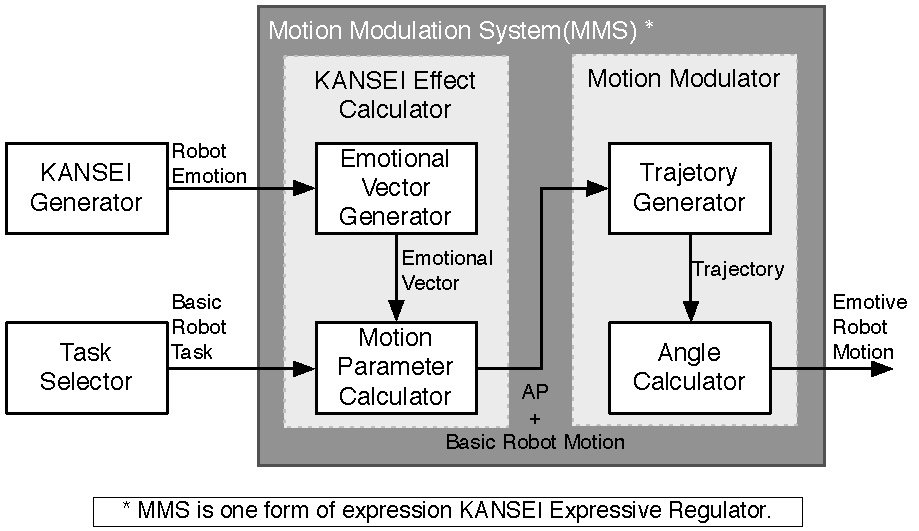
\includegraphics[height=7cm]{MMS.pdf}
%\vspace{-3mm}
\caption{PDF貼り付けの例:MMSの内部構成}
\label{fig:mms}
%\vspace{2mm}
\end{figure}

\subsection{図の位置の指定}
ここで,文章と文章の間などに図を入れたくなることがある.
これを制御する為の指定が,以下の部分である.
\begin{breakbox}
{\small
\begin{verbatim}
\begin{figure}[htbp]
\end{verbatim}
}
\end{breakbox}
「\verb+[htbp]+」の記載は,図を入れず場所の優先順位を「\verb+h+:ここに」「\verb+t+:ページ上部に」「\verb+b+:ページ下部に」「\verb+p+:1ページに」するという意味である.
状況に応じて,「\verb+[tb]+」「\verb+[ht]+」「\verb+[p]+」のように指定できる.
しかしながら,\LaTeX の場合,バランスがとれる位置に図を入れる為に,その出力位置を完全にはコントロールできないので,参照した場所より下に図が入っていれば良いぐらいの気持ちで良い.

ただし,今回のパッケージでは,float スタイルを組み込んでいる.
標準の \LaTeX にはない 「\verb+[H]+」オプションを使うことによって,強制的にその場に入れることができる.

\begin{breakbox}
{\small
\begin{verbatim}
\begin{figure}[H]
\centering
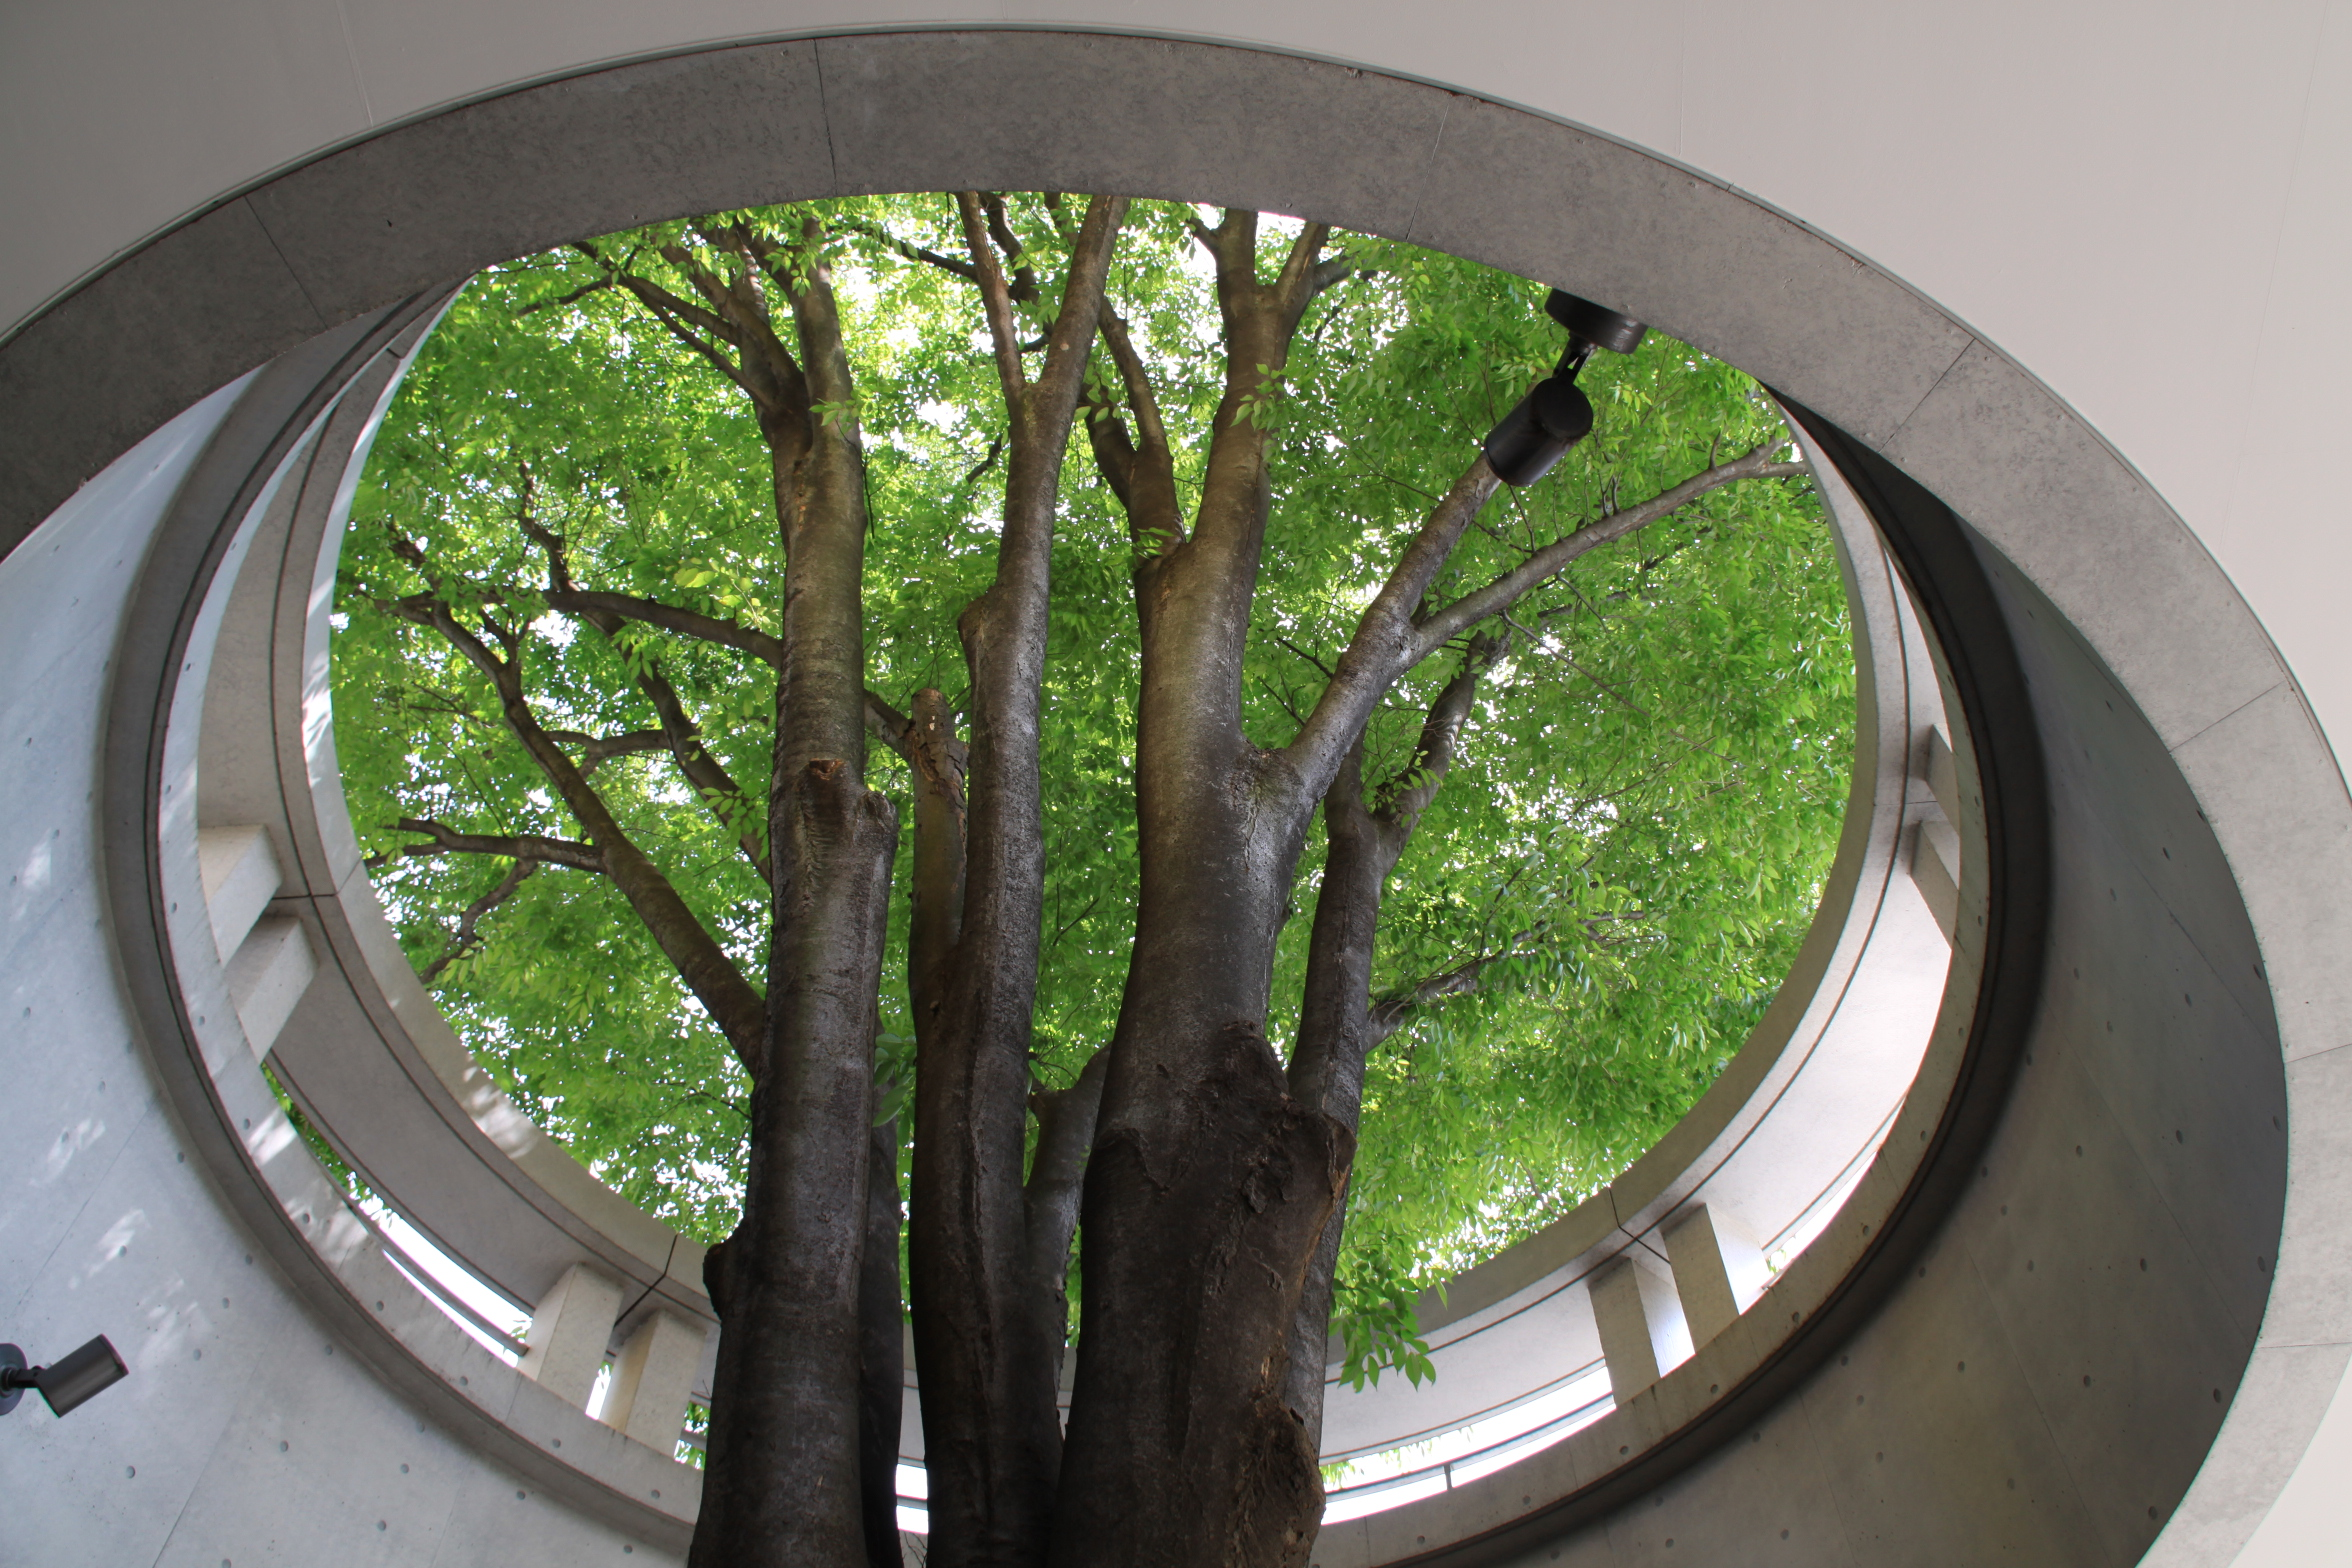
\includegraphics[height=5cm]{DEF059.jpg}
\caption{JPEG貼り付けの例:学内の写真}
\label{fig:sagamiC}
\end{figure}
\end{verbatim}
}
\end{breakbox}

\begin{figure}[H]
\centering
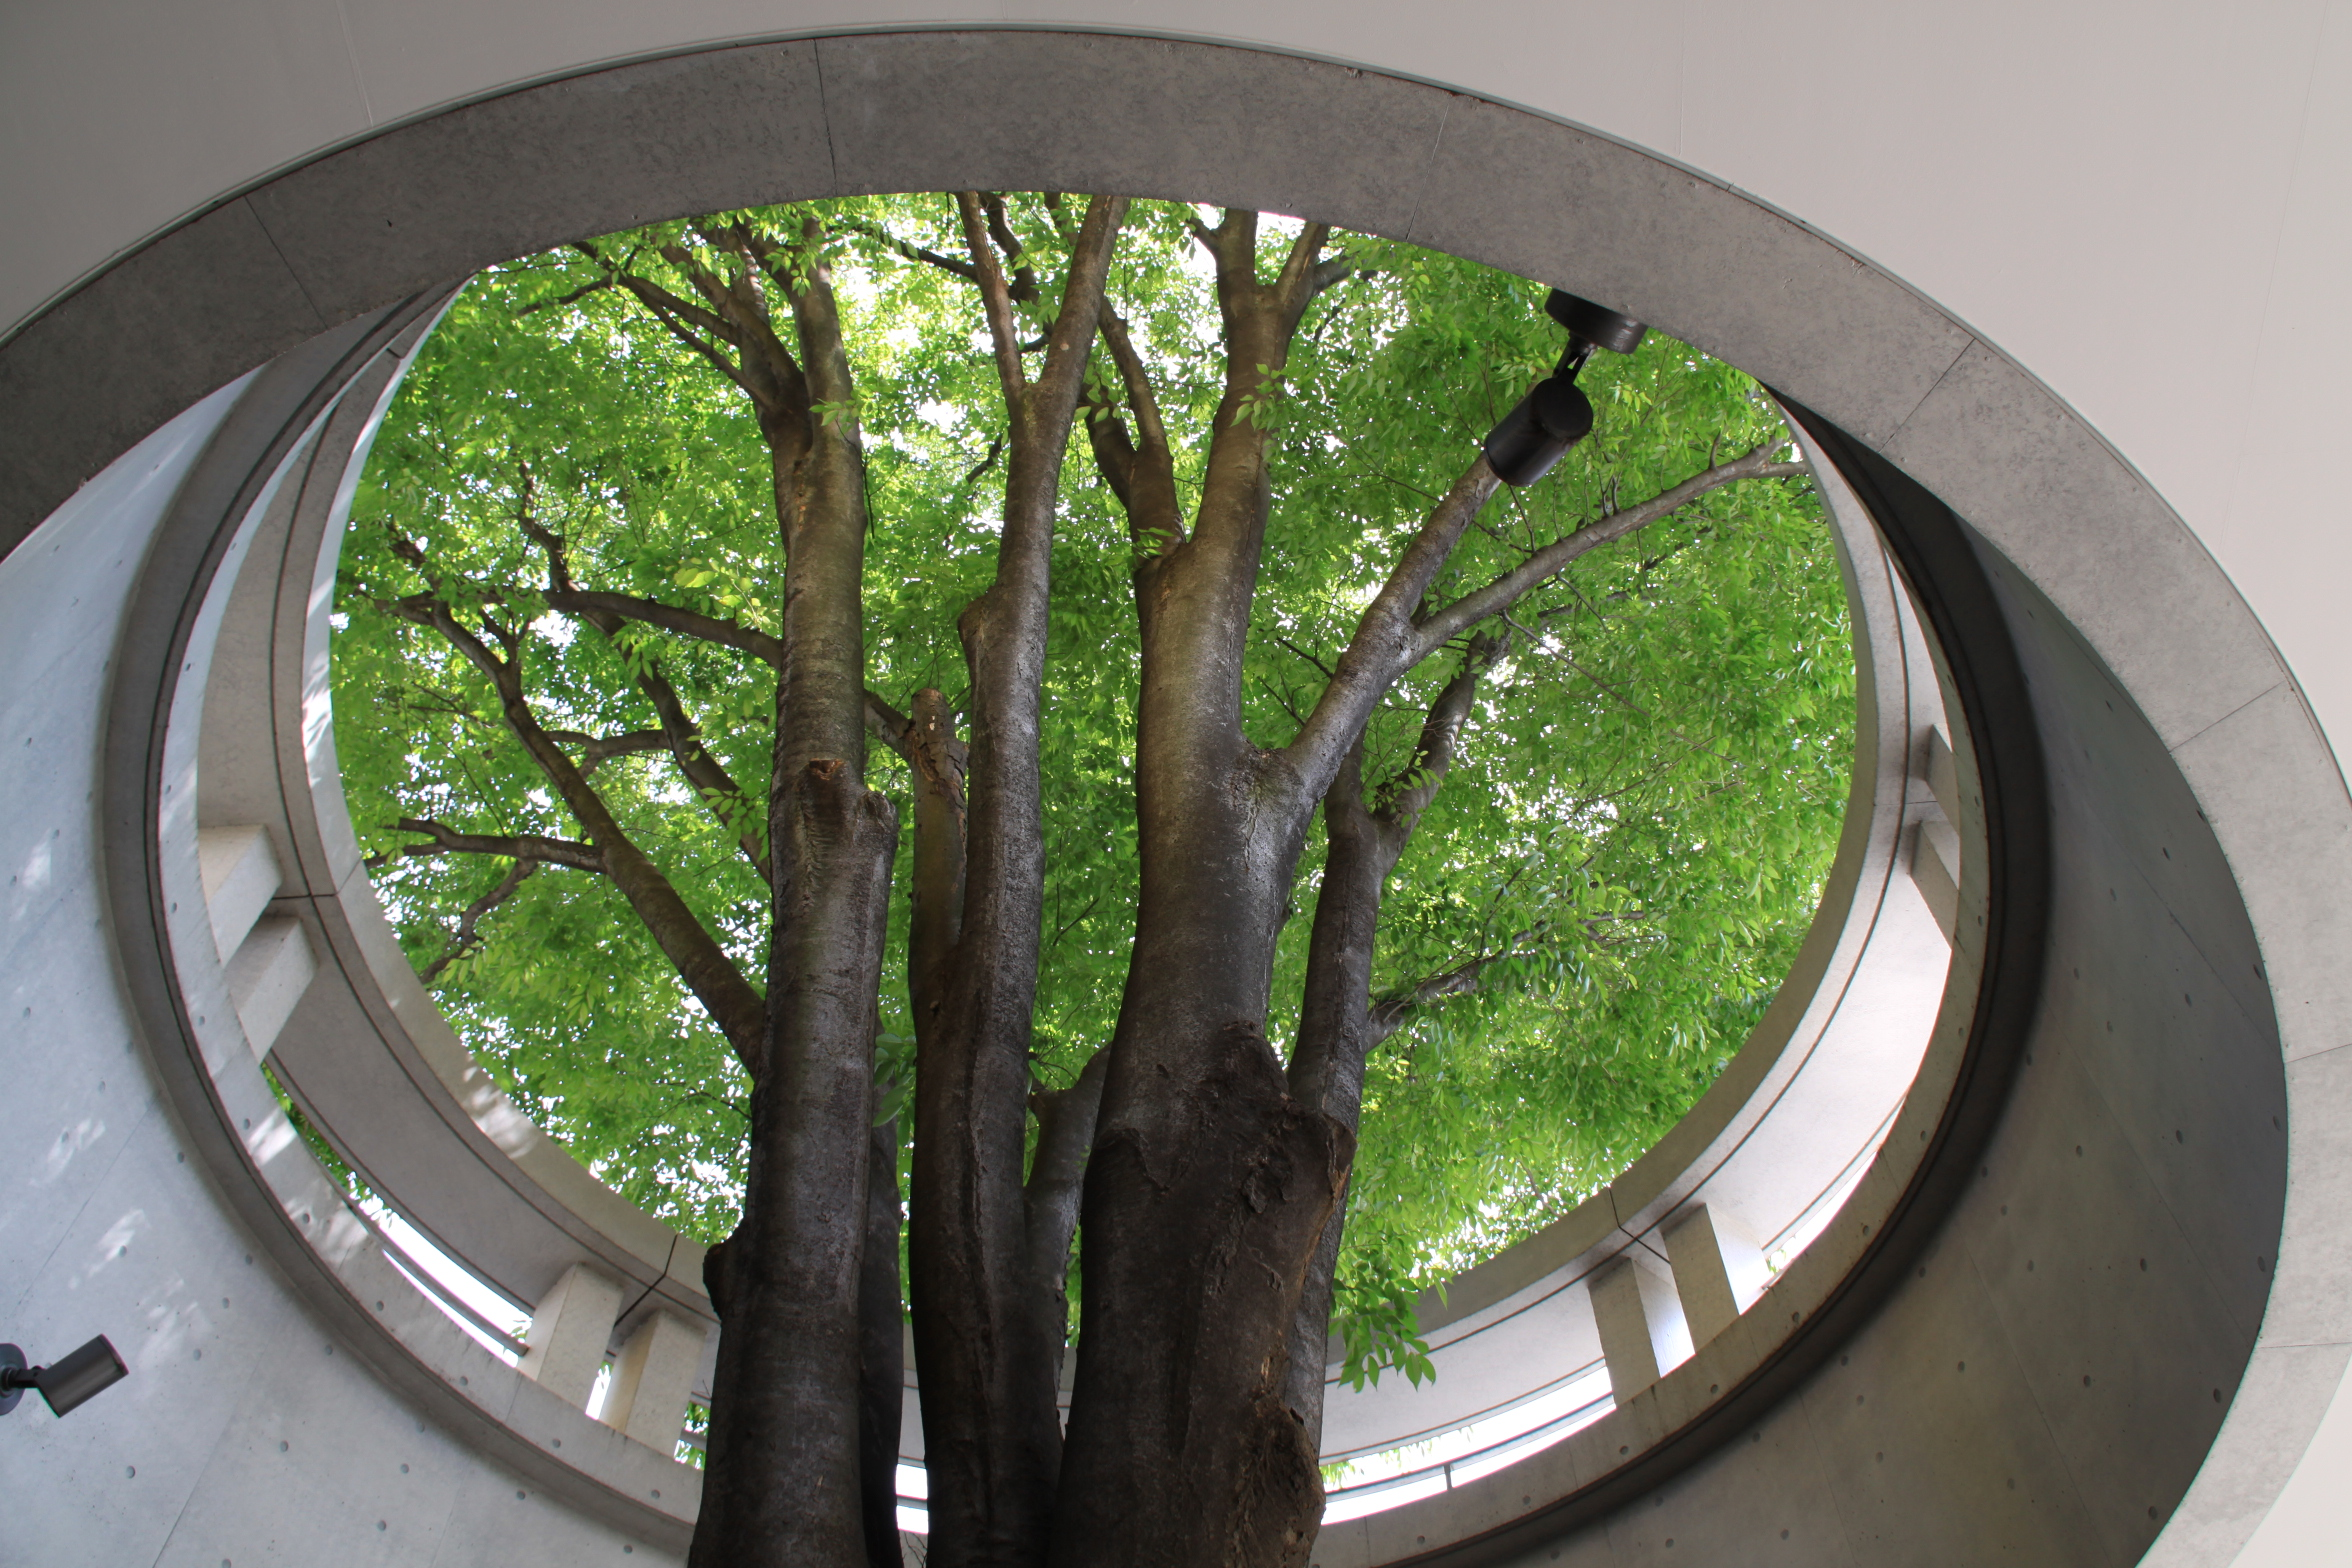
\includegraphics[height=5cm]{DEF059.jpg}
%\vspace{-3mm}
\caption{JPEG貼り付けの例:学内の写真}
\label{fig:sagamiC}
%\vspace{2mm}
\end{figure}

\subsection{図の参照}
図の挿入の際に(先ほど)記入した \verb+\label{fig:mms}+ は,図番号を参照したい際に指定するラベルを設定していた.
これを参照するには,「\verb+図 \ref{fig:mms}+」と指定すれば,図 \ref{fig:mms} の様に出力される.

\subsection*{補足:PDF, JPEG, PNG形式の場合の注意}
図の大きさを知らせる xbbファイルが必要になる.
これは,extractbbコマンドにて生成可能である.
本パッケージでは,\verb+mklatex.bat+ ファイルにて自動生成するように設定したため,あまり気にせず正しいファイル名のみ指定すれば良い.


